\documentclass[onecolumn,preprintnumbers,amsmath,amssymb,notitlepage,nofootinbib,longbibliography,superscriptaddress]{revtex4-1}
%\documentclass[preprint,showpacs,preprintnumbers,amsmath,amssymb]{revtex4}

\usepackage{natbib}
\usepackage{graphicx}
\usepackage{dcolumn}
\usepackage{dsfont}
\usepackage{bm}
%\usepackage{float}

\usepackage{xcolor}
\usepackage{url}
\usepackage[colorlinks=true,breaklinks=true,allcolors=blue]{hyperref}
\usepackage{microtype}
\DeclareMathOperator{\dist}{\text{dist}}

\newtheorem{theorem}{Theorem}
\newtheorem{lemma}{Lemma}

\newcommand{\ryan}[1]{\textcolor{cyan}{#1}}



\begin{document}

\title{DeepQ Decoding for Fault Tolerant Quantum Computation}

\author{Ryan Sweke}
\affiliation{\mbox{Dahlem Center for Complex Quantum Systems, Freie Universit\"{a}t Berlin, 14195 Berlin, Germany}}
\author{Markus Kesselring}
\affiliation{\mbox{Dahlem Center for Complex Quantum Systems, Freie Universit\"{a}t Berlin, 14195 Berlin, Germany}}
\author{Evert P.L. van Nieuwenburg}
\affiliation{\mbox{Institute for Quantum Information and Matter, Caltech, Pasadena, CA 91125, USA}}
\author{Jens Eisert}
\affiliation{\mbox{Dahlem Center for Complex Quantum Systems, Freie Universit\"{a}t Berlin, 14195 Berlin, Germany}}


\date{\today}


\begin{abstract}
Topological error correcting codes, and particularly the surface code, currently provide the most feasible roadmap towards large-scale fault tolerant quantum computation. As such, obtaining fast and flexible decoding algorithms for these codes, within the experimentally relevant context of faulty syndrome measurements, is of critical importance. In this work we show that the problem of decoding such codes, in the full fault tolerant setting, can be naturally reformulated as a process of repeated interactions between a decoding agent and a code environment, to which the machinery of reinforcement learning can be applied to obtain decoding agents. As a demonstration, by using deepQ learning, we obtain fast decoding agents for the surface code, for a variety of noise-models, within the fully fault tolerant setting.
\end{abstract}

\maketitle
 
 
\section{Introduction}\label{s:introduction}

    In order to implement large scale quantum algorithms it is necessary to be able to store and manipulate quantum information in a manner that is robust with respect to the unavoidable errors introduced through the interaction of physical qubits with a noisy environment. A typical strategy for achieving such robustness is to encode a single logical qubit into the state of many physical qubits, via a quantum error correcting code, from which it may be possible to actively diagnose and correct errors that might occur. While many quantum error correcting codes exist, topological quantum codes in which only local operations are required to diagnose and correct errors, are of particular interest as a result of their experimental feasibility. Recently the surface code has emerged as an espescially promising code for large scale fault tolerant quantum computation, due to the combination of its comparitively low overhead and locality requirements, coupled with the availability of convenient strategies for the implementation of all required logical gates.

    Within any such code based strategy for fault tolerant quantum compuation, decoding algorithms play a critical role. At a high level, throughout the course of a computation these algorithms take as input the outcome of diagnostic syndrome measurements and should provide as output suggested corrections for any errors which might have occured, which can then be tracked through the computation and later used to apply corrections to any obtained results. It is particularly important to note that in any physically realistic setting the required syndrome measurements are themselves obtained via small quantum circuits, and are therefore also generically faulty. As such, while the setting of perfect syndrome measurements provides a good test-bed for the development of decoding algorithms, any decoding algorithm which aims to be experimentally feasible should also be capable of dealing with such faulty syndrome measurements. Additionally, such algorithms should also be capable of dealing with experimentally relevant noise models, as well as be fast enought to not present a bottleneck to the execution of computations, even as the size of the code scales to larger code distances.

    Due to the importance of decoding algorithms for fault tolerant quantum computation, many different approaches have been developed, each of which tries to satisfy as many of the experimentally required criterion as possible. Perhaps most prominent are algorithms based on minimum-weight perfect matching subroutines, however alternative approaches based on techniques such as the renormalization group and locally operating cellular automata have also been put forward. Furthermore, recently techniques from classical machine learning have begun to find application in diverse areas of quantum physics - such as in the efficient representation of many-body quantum states, the identification of phase transitions, and the autonomous design of novel experimental setups - and various neural-network based decoders have also been proposed. However, despite the diversity of decoding algorithms now available, there is not as of yet an algorithm which clearly satisifes all the required criteria, or a clear consensus as to which technique would be the most experimentally feasible in any given experimental context. In particular, while the so-far proposed neural network decoders promise extremely fast decoding times, flexibility with respect to the underlying noise model and the potential to scale to large code distances, all such decoders are so far restricted either to the setting of perfect syndrome measurements, or to the setting in which one is trying to store a logical qubit as long as possible, without the requirement of performing a subsequent logical gate.  As such, while this approach seems promising, there remains room for improvement and generalization.

    Simultaneously, the last few years have also seen extremely impressive advances in the development of deep reinforcement learning algorithms, which have allowed for the training of neural network based agents capable of obtaining super-human performance in domains such as Atari, Chess and Go. These techniques are particularly powerful in situations where it is necessary to learn strategies for complex sequential decision making, involving consideration of the future effects of ones actions. At a surface level, the problem of decoding within the context of fault-tolerant quantum computation seems like exactly such a setting and as such it natural to ask to what extent reinforcement learning techniques could be used to obtain decoding agents, and what advantages such agents might have over existing approaches. In this work we set out to provide answers to these questions.

    In particular, we reformulate the problem of decoding within the setting of fault-tolerant quantum computation as a process of sequential competitive interaction between a decoding agent and a code environment. This reframing provides a conceptual framework which allows for the application of various deep reinforcement learning algorithms to obtain neural network based decoding agents. As a proof-of-principle, we then utilize to deepQ learning to obtain fast surface code decoders, for a variety of noise models, within the fully fault-tolerant setting. These results then provide a foundation for extension via both more sophisticated reinforcement learning techniques and more sophisticated neural network models.

    In this work we begin by providing an introductory overview of the surface code in Section \ref{s:the_surface_code}, before presenting a description of the decoding problem for fault-tolerant quantum computation in Section \ref{s:the_decoding_problem}. After a brief introduction to the formalism of reinforcement learning and $Q$-functions in Section \ref{s:reinforcement_learning} we are then able to provide the conceptual reframing of decoding as a reinforcement learning problem in Section \ref{s:decoding_as_rl}, which is one of the primary results of this work. In Section \ref{s:results} we then present deepQ surface code decoders for a variety of noise models, before finally in Section \ref{s:conclusions} discussing both the advantages and disadvantages of the approach presented here, along with various potential strategies for building upon the results presented in this work.



\section{The Surface Code}\label{s:the_surface_code}


    We begin by providing a brief high-level and hopefully intuitive description of the surface code. The framework and methods presented in this work are not restricted to the surface code, and could be applied to any stabilizer code, but we choose to restrict ourselves to this code here for both simplicity of presentation and experimental relevance. We will focus here on presenting the elements of the surface code necessary for understanding the decoding problem that we aim to address, in the process omitting many details, however there exists a rich underlying theory to both topological error correcting codes, and stabilizer codes more generally, and for a more rigorous or condensed matter perspective we refer to the refs \textit{a,b, and c}.

    As illustrated in Fig. \ref{f:surface_code}, we will consider $d\times d$ lattices with a \textit{data qubit} on each vertex, such that states of the lattice are elements of the Hilbert space $\mathcal{H} = \bigotimes_{v \in V}\mathbb{C}^2$, where we have indicated the set of all vertices as $V$. A surface code on such a lattice is defined by a set $S$ of plaquette stabilizer operators, of which there are four distinct types; Given single-qubit Pauli operators $X$ and $Z$, bulk (boundary) plaquette stabilizers $X_{p}$ and $Z_{p}$ are local four (two) body operators,

    \begin{equation}
        X_{p} \equiv \bigotimes_{q \in p} X_q, \quad Z_{p} \equiv \bigotimes_{q \in p} Z_q,
    \end{equation}
    which act non-trivially only on the vertex qubits of plaquette $p$. With reference to Fig \ref{f:surface_code}, if we denote the set of all blue (orange) plaquettes as $B_p$ ($O_p$), then the set $S$ of stabilizers defining the surface code is given by,

    \begin{equation}
        S = \big\{ X_p \vert p \in B_p  \big\} \cup \big\{ Z_p \vert p \in O_p  \big\},
    \end{equation}
    from which we can define the Hamiltonian of the surface code as $H_{\mathrm{sc}} \equiv -\sum_{\hat{O} \in S}\hat{O}$. 

    At this point it is possible to understand how we can encode one \textit{logical qubit} into the surface code. We begin by defining the \textit{code space} $\mathcal{H}_{\mathrm{sc}}$ as the ground state space of the surface code Hamiltonian $H_{\mathrm{sc}}$. This code space contains all surface code states $|\psi\rangle \in \mathcal{H}$ which are simultaneous $+1$ eigenstates of all stabilizers $\hat{O} \in S$ - i.e. states which commute with all stabilizers in $S$. A simple counting arguement allows one to verify that this code space is in fact two-dimensional - i.e. $\mathcal{H}_{\mathrm{sc}} \simeq \mathbb{C}^2$ - such that we can effectively identify the code space with the state space of a single qubit, which is the logical qubit associated with the surface code. In addition, as illustrated in Fig. \ref{f:surface_code}, let us define $Z_L$ ($X_L$) as any continuous string of single vertex $Z$ ($X$) operators connecting the left and right (top and bottom) boundaries of the code. Despite the fact that these \textit{logical operators} cannot be expressed as the product of stabilizer operators in $S$, the eigenstates of these operators are elements of the code space, and these operators map states in the code space into other states in the code space. As such, we see that we can use the eigenstates $\{ |0_L\rangle, |1_L\rangle \}$ of $Z_L$ to define a basis for the code space, and additionally, given a state within the code space, i.e. a state of the logical qubit, we can manipulate this state by using products of logical operators. 

      \begin{figure}
      \centering
          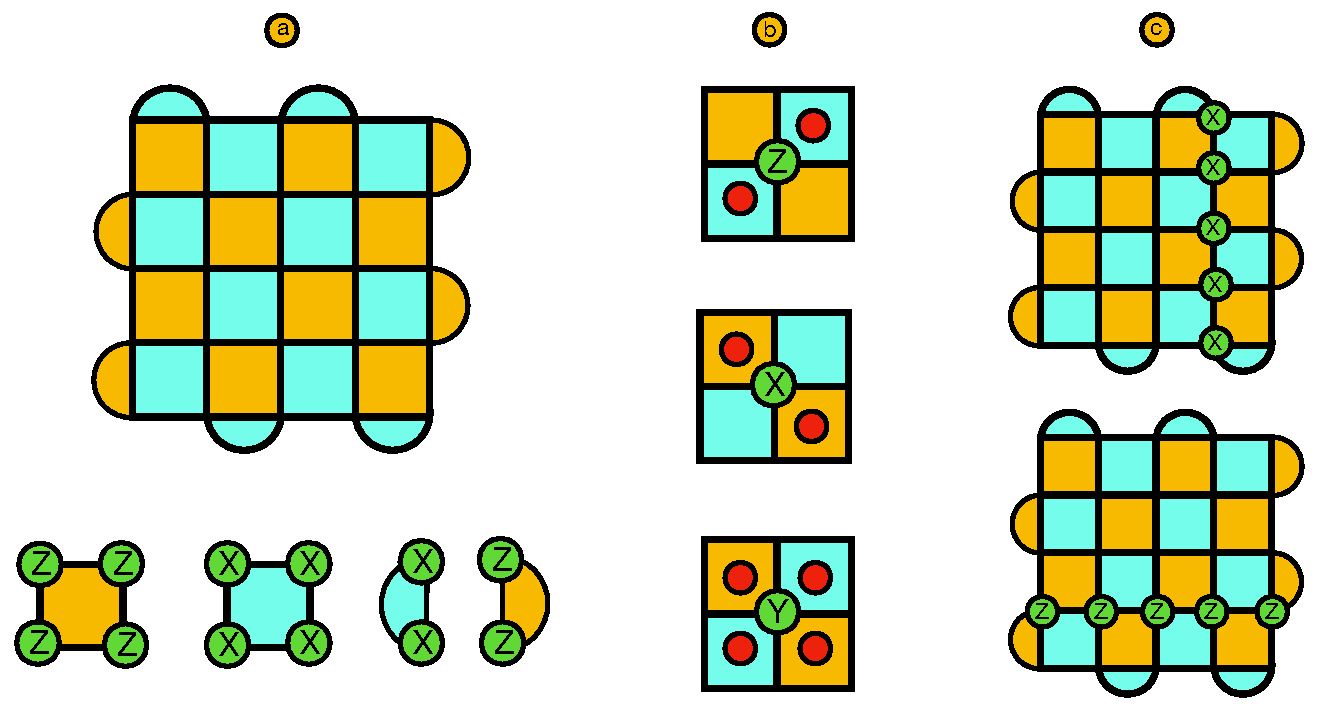
\includegraphics[width=0.75\textwidth]{surface_code.pdf}
      \caption{An overview of the surface code. (a) We consider square $d\times d$ lattices, with a data qubit on each vertex of the lattice. Additionally, there exist four types of local stabilizer operators: bulk $X$ ($Z$) stabilizers, which are four-body operators acting on the vertex qubits of blue (orange) plaquettes in the bulk of the lattice, and boundary $X$ ($Z$) stabilizers, which are two-body operators acting on the vertex qubits of blue (orange) plaquettes on the boundary of the lattice. (b) Assuming that each data qubit is initialized in the $+1$ eigenstate of the single-qubit $Z$ operator, single qubit Pauli flips on vertex qubits will cause the global lattice state to anti-commute with certain stabilizers supported on this vertex. Here we have illustrated the stabilizers \textit{violated} (those which anti-commute with the global lattice state) after different Pauli flips are applied to a single data qubit. (c) Logical $X_L$ and $Z_L$ operators for the surface code are provided by continuous strings of single qubit $X$ or $Z$ operators connecting the top and bottom or left and right boundaries of the code respectively.}\label{f:surface_code}
    \end{figure}

    At this point it is natural to ask for the motivation behind such a redundant encoding. To answer this question, let's assume that the global lattice state $|\psi\rangle$ is an element of the code space - i.e. a simultaneous $+1$ eigenstate of all the stabilizer operators in $S$. In the process of storing (or manipulating) this state it may happen that some unavoidable error or noise process causes an operation, such as a single qubit Pauli flip on a single data qubit, which is not a logical operation, and therefore causes the global lattice state to move outside of the code space. At this point, the global lattice state \textit{will not} commute with all the stabilizers, and will instead anti-commute with some of the stabilizers supported on the flipped data-qubit (as illustrated in Fig. \ref{f:surface_code}). If we define a \textit{syndrome} as a binary string encoding the outcome of a simultaneous measurement of all the stabilizers in $S$, then we can see that the syndrome obtained from the global lattice state after the single qubit Pauli flip will contain a $-1$ entry in each position corresponding to a stabilizer with which the global lattice state anti-commutes, and $+1$ entries everywhere else. We say that stabilizers which anti-commute with the global lattice state are \textit{violated}. As we will discuss in detail in the next section, unlike a truly single qubit encoding of the state $|\psi\rangle$, there is now a chance that from the measured syndrome we will be able to diagnose the error which occured and implement a correction which moves the global lattice state back into the code space. 



\section{The Decoding Problem}\label{s:the_decoding_problem}

    % \begin{figure}
%   \centering
%       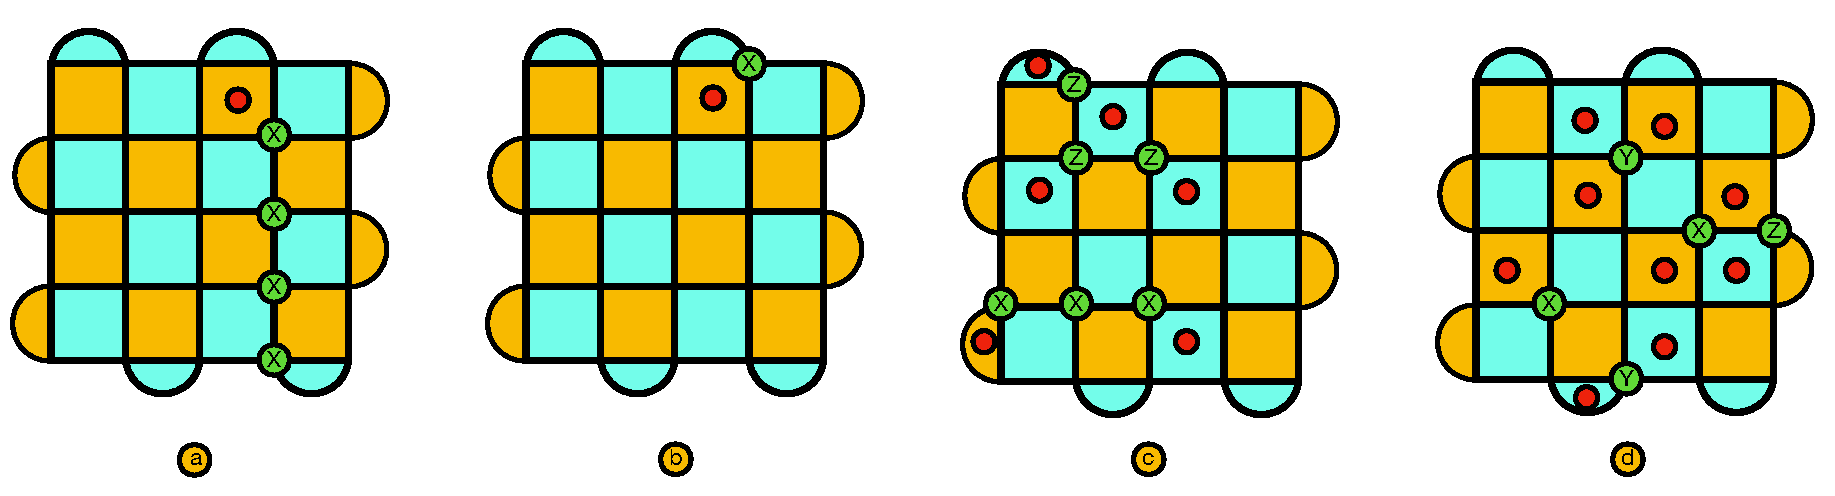
\includegraphics[width=0.75\textwidth]{surface_code_examples.pdf}
%   \caption{A picture of the same gull
%            looking the other way!}
% \end{figure}
\section{Reinforcement Learning and Q-Functions}\label{s:reinforcement_learning}
\section{Decoding as a Reinforcement Learning Problem}\label{s:decoding_as_rl}
\section{Results}\label{s:results}
\section{Conclusion}\label{s:conclusions}


\begin{acknowledgments}
The authors gratefully acknowledge helpful and insightful discussions with Daniel Litinski, Nicolas Delfosse and Hendrik Poulsen Nautrup. Additionally, the authors would like to thank J\"{o}rg Behrmann for incredible technical support, without which this work would not have been possible. R.S.\ acknowledges the financial support of the Alexander von Humboldt foundation.
\end{acknowledgments}	

\bibliography{dq}

\end{document}
